\documentclass[border=10pt]{standalone}
\usepackage{pgfplots}
\pgfplotsset{compat=newest}
\begin{document}
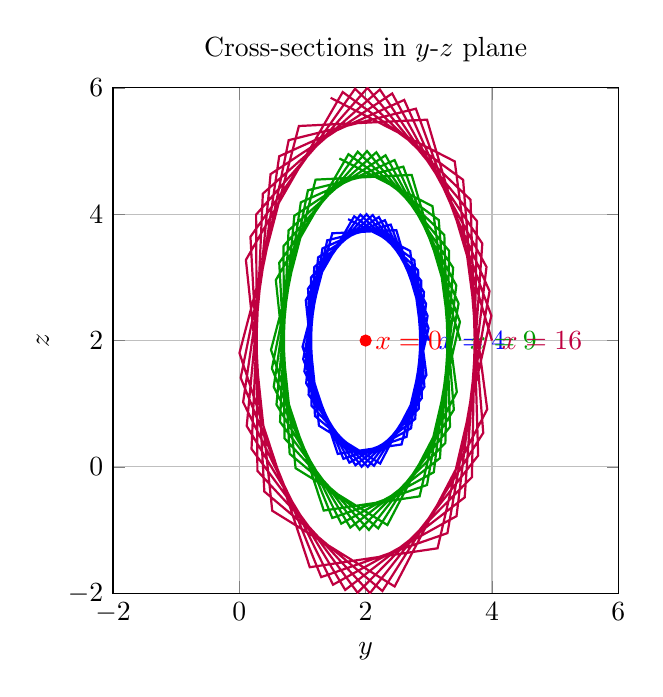
\begin{tikzpicture}
\begin{axis}[
    xlabel={$y$},
    ylabel={$z$},
    title={Cross-sections in $y$-$z$ plane},
    grid=major,
    axis equal image,
    xmin=-2, xmax=6,
    ymin=-2, ymax=6,
    width=8cm,
    height=8cm
]
% x = 0: point (2,2)
\addplot[only marks, mark=*, red] coordinates {(2,2)};
\node[red, anchor=west] at (axis cs:2,2) {$x=0$};

% x = 4: (y-2)^2 + (z-2)^2/4 = 1
\addplot[blue, thick, domain=0:360, samples=50] ({2 + cos(deg(x))}, {2 + 2*sin(deg(x))});
\node[blue, anchor=west] at (axis cs:3,2) {$x=4$};

% x = 9: (y-2)^2/(9/4) + (z-2)^2/9 = 1
\addplot[green!60!black, thick, domain=0:360, samples=50] ({2 + 1.5*cos(deg(x))}, {2 + 3*sin(deg(x))});
\node[green!60!black, anchor=west] at (axis cs:3.5,2) {$x=9$};

% x = 16: (y-2)^2/4 + (z-2)^2/16 = 1
\addplot[purple, thick, domain=0:360, samples=50] ({2 + 2*cos(deg(x))}, {2 + 4*sin(deg(x))});
\node[purple, anchor=west] at (axis cs:4,2) {$x=16$};

\end{axis}
\end{tikzpicture}
\end{document}
